\documentclass[12pt,oneside]{report}

%%% Load some useful packages:
%% "New" LaTeX2e graphics support.
\usepackage{graphicx}
%%	using final option to force graphics to be included even in draft mode
%\usepackage[final]{graphicx}
%% Tell graphicx the default directory for all figures
\graphicspath{{figures/}}

% Enable subfigure support
\usepackage{subfigure}

%% Make subsubsections numbered and included in ToC
\setcounter{secnumdepth}{3}
\setcounter{tocdepth}{2}

%% Package to linebreak URLs in a sane manner.
\usepackage{url}

%% Define a new 'smallurl' style for the package that will use a smaller font.
\makeatletter
\def\url@smallurlstyle{%
  \@ifundefined{selectfont}{\def\UrlFont{\sf}}{\def\UrlFont{\small\ttfamily}}}
\makeatother
%% Now actually use the newly defined style.
\urlstyle{smallurl}

%% Define 'tinyurl' style for even smaller URLs (such as in tables)
\makeatletter
\def\url@tinyurlstyle{%
  \@ifundefined{selectfont}{\def\UrlFont{\sf}}{\def\UrlFont{\scriptsize\ttfamily}}}
\makeatother

%% Provides additional functionality for tabular environments
\usepackage{array}

%% Puts space after macros, unless followed by punctuation
\usepackage{xspace}

%% Make margins less ridiculous
\usepackage{fullpage}

%% Allows insertion of fixme notes for future work
\usepackage[footnote, nomargin]{fixme}

%%%% Turned off for tech report, should be turned on for research portfolio
%% Turn on double spacing
\usepackage{setspace}
\usepackage{mdwlist}
\doublespacing

%% Make URLs clickable
%\usepackage[colorlinks, bookmarks=false]{hyperref}
\usepackage[colorlinks, bookmarks=true]{hyperref}

%% Since I'm using the LaTeX Makefile that uses dvips, I need this
%% package to make URLs break nicely
\usepackage{breakurl}

\usepackage{todonotes}
\usepackage{amsmath,amsfonts}
\numberwithin{equation}{subsection}
%%\usepackage{nonfloat}
\usepackage{bbm}
\usepackage{setspace}
\onehalfspacing
\usepackage{tabularx}

\newenvironment{myindentpar}[1]%
 {\begin{list}{}%
         {\setlength{\leftmargin}{#1}}%
         \item[]%
 }
 {\end{list}}

%%% End of preamble
\begin{document}

\begin{titlepage}

\begin{center}

\tiny{.}\\ [1.2cm]

\Large{Dissertation draft:} \\ [0.5cm]
\LARGE{\textsc{Software Trajectory Analysis:}} \\
\LARGE{\textsc{An empirically based method for automated software process discovery}} \\ [0.6cm]

\large{
Pavel Senin \\
Collaborative Software Development Laboratory \\
Department of Information and Computer Sciences \\
University of Hawaii \\
\texttt{senin@hawaii.edu} \\ [1.0cm]


\emph{Committee:} \\
Philip M. Johnson, Chairperson \\
%%Kyungim Baek \\
%%Guylaine Poisson \\
%%Henri Casanova \\
%%Daniel Port \\ [1.5cm]
}

\normalsize{
CSDL Technical Report 09-14 \\
\url{http://csdl.ics.hawaii.edu/techreports/09-14/09-14.pdf} \\ [1.5cm]
}

\large{2012}

\end{center}

\end{titlepage}


%% Philip suggests it needs a ToC
\tableofcontents

%%%%%%%%%%%%%%%%%%%%%%%%%%%%%% -*- Mode: Latex -*- %%%%%%%%%%%%%%%%%%%%%%%%%%%%
%% uhtest-abstract.tex -- 
%% Author          : Robert Brewer
%% Created On      : Fri Oct  2 16:30:18 1998
%% Last Modified By: Robert Brewer
%% Last Modified On: Fri Oct  2 16:30:25 1998
%% RCS: $Id: uhtest-abstract.tex,v 1.1 1998/10/06 02:06:30 rbrewer Exp $
%%%%%%%%%%%%%%%%%%%%%%%%%%%%%%%%%%%%%%%%%%%%%%%%%%%%%%%%%%%%%%%%%%%%%%%%%%%%%%%
%%   Copyright (C) 1998 Robert Brewer
%%%%%%%%%%%%%%%%%%%%%%%%%%%%%%%%%%%%%%%%%%%%%%%%%%%%%%%%%%%%%%%%%%%%%%%%%%%%%%%
%% 

\begin{abstract}
Abstract goes here, and will be written once the proposal is mostly done.
\end{abstract}


% my main text chapters
\chapter{Introduction}\label{chapter_introduction}
\textit{The central issue I address in the dissertation is a possibility of recurrent behaviors discovery from 
publicly available software process artifacts by leveraging data mining and knowledge discovery techniques. 
In particular I explored an approach of discovering of recurrent behaviors through the mining of time series that
are constructed by temporal ordering of measurements extracted from software process artifacts.
Further, I shall propose a novel technique for characteristic patterns discovery from time series and show its 
applicability to the problem at hands.}

\textit{The problem's background is provided in the Section \ref{section_background}. 
Section \ref{section_software_process_design} presents classical approaches for software process design and shows its limitations.
Section \ref{section_research_hypothesis} introduces the research hypothesis.
Section \ref{knowledge_discovery} provides a background into the problem of knowledge discovery 
from time-series.
Section \ref{section_trajectory_definition} connects two problems and provides definitions.
Section \ref{section_contributions} enumerates main contributions of the thesis, 
while section \ref{section_organization} explains the thesis organization.}

%
% >> section
%
\section{Background}\label{section_background}
Contemporary software projects concern with development of complex software systems and typically have 
a considerably long life-cycle - well over decade.
A project's development and maintenance activities are usually carried out by geographically 
distributed teams and individuals. The development pace, the experience, and the structure of the 
development team continuously change with project progression and as developers joining and leaving. 
When combined with schedule and requirements adjustments, these create numerous difficulties 
for developers, users, and stakeholders, ultimately affecting the project success \cite{citeulike:2207657}. 

This software development complexity phenomena was identified in 1968 as ``Software crisis'' 
\cite{naur_crisis_68}, and was addressed by bringing the research and the practice of software development 
(or as it was called ``programming'') under the umbrella of Engineering - in an effort to provide 
the control over the process of software development. 
Following the engineering paradigm, numerous methodologies and models of software design and development 
process, known as \textit{software processes}, were proposed \cite{citeulike:10002165}.

\begin{defn}\label{def_process}
A \textbf{\textit{Software Process}} defines a sequence of activities performed in order 
to design, develop, and maintain software systems.
\end{defn}
Examples of such activities include requirements collection and creation of UML diagrams, 
requirements testing, code development,  testing, etc. The intent behind a software process is 
to provide a control over software evolution by implementing a global strategy and by structuring
and coordinating human activities in order to achieve the goal - deliver a functional software system 
on time and under the budget. 

Since then, much research has been done on software processes resulting in a number
of software development models and paradigms. Some of these were widely accepted by practitioners 
and evolved into industrial standards for software development processes such as CMM, ISO, PSP, 
and others \cite{citeulike:5043104}. However, in spite of this effort, industrial software 
development remains error-prone and more than half of all 
commercial software development projects ending up failing or being very poorly executed 
(Rubinstein, ``Chaos Reports'', 2006) \cite{chaos2006}. Some of them are abandoned due to running 
over budget, some are delivered with such low quality, or so late, that they are useless, and some, 
when delivered, are never used because they do not fulfill requirements. 

Through the analyses of software project failures, it was acknowledged, that the engineering 
paradigm might not be the best way to provide a control over software development processes 
(\cite{citeulike:3729379} \cite{citeulike:5203446}) due to the fact that Software engineering 
is dealing with significantly different from other Engineering fields problems \cite{citeulike:2207657} .
The chief argument supporting this point of view is the drastic difference in the cost model:
while in Software Engineering there is almost no cost associated with materials and 
fabrication, these usually dominate cost in all other Engineering disciplines, but, 
ironically, Software Engineering is suffering from the costs and challenges associated with 
continuous re-design of the product and its design processes - the issue which is 
hardly seen at all in other Engineering areas. 
Further, it was found, that most of the engineering-like models are rigid, ``context-free'',
and rather prescriptive, i.e. they are universally defined independently of a particular 
organizational structure or a project specificities \cite{sacchi_2001}, and while they 
structure processes and provide the control, following them does not guarantee the success.
Yet another argument supporting alternative to engineering approaches is the increasing 
understanding and appreciation of a human role in software development processes over tools, 
technologies, and standards \cite{citeulike:6580825} \cite{citeulike:149387}
\cite{1605185} \cite{citeulike:113403} \cite{1605188} \cite{citeulike:12743107}. 

Along with Software Engineering, a number of alternative, flexible and user-oriented software processes 
emerged from academy, hobbyists, and practitioners addressing aforementioned issues \cite{citeulike:3729379}. 
Among others, the Free/Libre/Open-Source Software model (FLOSS) and the software craftsmanship  
approaches gained a significant credibility in community. 
While the former \textit{holistic} software process paradigm emphasizes loosely-organized 
collaboration, frequent releases, and effectively removes the boundary between developers 
and customers, the latter, human-centric approach, is built upon the roles of highly 
motivated skilled individuals \cite{citeulike:262020} \cite{citeulike:2759198}. 

Nevertheless, alternative processes were found to be plagued by the same complexity issues. 
As it was shown, most of FLOSS projects never reach a ``magic'' 1.0 version \cite{citeulike:12480029}. 
Among others, the great "infant mortality rate" of FLOSS projects was related to a burnout, 
inability to acquire a critical mass of users, loss of leading developer(s), and forking \cite{richter2007critique}. 
Software craftsmanship, from other hands, not only challenges developers with technological advances 
requiring continuous skills improvement, but creates significant cost and effort estimation difficulties for
stakeholders and project managers \cite{citeulike:11058784}. However, despite to these issues, 
the alternative processes proved that the disciplined manner of programming and the modularization  
of the software are capable of delivering large and reliable software systems, most notable Linux OS,
suggesting that community-driven processes as good as industrial engineering-like processes.

Currently, it is widely acknowledged, that there exists no single ``silver bullet'' process which 
can bring a software development project to success \cite{citeulike:1986013}. 
Processes are numerous, each has advantages and drawbacks, and each is accompanied with 
numerous application recommendations, success stories, and with failure experiences. Nevertheless,
the alarming rate of failing projects suggests that our understanding of software process ``mechanics''  
is limited and insufficient\cite{citeulike:12550665}. 
The enormous cost of the lost effort, measured in hundreds of billions of US dollars 
\cite{citeulike:2207657} \cite{citeulike:2207653} \cite{citeulike:2207655}, 
continues to provide motivation for further research on software processes. 

%
% >> section
%
\section{Software process design}\label{section_software_process_design}
Traditionally, approaches to software process design and improvement are divided into two distinct categories. 

The first category of software process design approaches consists of traditional to engineering 
\textit{top-down} prescriptive techniques through 
\textit{proposing a process based on specific patterns of software development}. 
For example, the Waterfall Model process proposes a sequential pattern in which developers first create a 
Requirements document, then create a Design, then create an Implementation, and finally develop Tests. 
The Test Driven Development process, from other hands, proposes an iterative behavioral pattern in which
the developer must first write a test case, then write the code to implement that test case, then re-factor the 
system for maximum clarity and minimal code duplication \cite{citeulike:6086365}. 

While the top-down approach follows the usual path of trials and errors, and seems to be an extension 
of natural to humans creative processes of invention and experimentation, 
the ``invention'' of an adequate to the task software process is far from trivial 
\cite{citeulike:5043104} \cite{citeulike:1986013}. Moreover, an evaluation cycle of an invented process
is usually very expensive and considerably long.
In addition, it was shown that the process inventors are often limited in their scope and tend to assume 
idealized versions of real processes, thus, often produce ``paper lions'' - process models which are 
likely to be disruptive and unacceptable for end users, at least in their proposed form 
\cite{citeulike:9758924}, which creates a large discrepancy between actions that supposed to be done for 
the novel process and what was actually performed by particular individual or the team.

The second category of software design approaches consists of \textit{bottom-up} techniques 
that focus on a \textit{performed process reconstruction through noticing of recurrent development 
events and behaviors} or as it also called \textit{process enactment}. 
Usually, the process reconstruction task is viewed as a two-levels problem where the first level 
consists of a patterns discovery (segmentation) while the second level consists of patterns recognition 
and their network analysis \cite{citeulike:2703162}.
One of the first works in this category was by Cook and Wolf, where they show a
possibility of automated extraction of a process model through the mining of recorded 
process event logs \cite{citeulike:328044} \cite{citeulike:5120757} \cite{citeulike:5128143}. 
Later work by Huo et al. shows that it is also possible to improve an existing process
through the event logs analysis \cite{citeulike:7691059} \cite{citeulike:7690766}. 

While the bottom-up approaches seem to be more systematic and potentially less complex than invention, 
they also affected by a number of issues. A chief among these is the observability issue - 
it is usually very difficult to conduct a full depth study on a live project due to the privacy concerns. 
Moreover, it is expensive to observe a process performed by a team for a whole life-cycle of a project. 
Yet another issue is the capacity of currently available process discovery techniques - 
typically these need to be supervised by experts and finely tuned in order to reconstruct 
distributed and concurrent processes. 

Nevertheless, despite to their differences, both techniques for software process design are 
producing process models that effectively are the series of actions that must be performed successively 
(sequentially and sometimes iteratively) in order to deliver a software. 
In order to produce the viable model, the ``process inventors'' put the best of their knowledge, experience,
creativity, and logical reasoning into the proposed sequence of steps, while ``process re-constructors 
strive to eliminate the noise and to converge to a concise process model that is supported by the 
majority of observations. 
This attention to synthesis of sequential steps, leaves other phenomenas, such as team's structure, work schedule, 
developer's discipline, their behaviors, and motivation behind. While this issue was recognized previously
and resulted in a number of studies which called for attention of human element in software production 
\cite{citeulike:149387} \cite{citeulike:113403} \cite{citeulike:205322} \cite{citeulike:12798652}, 
it is still largely ignored in industrial practices \cite{citeulike:12798659}, mostly due to the 
difficulties in benefit estimation \cite{citeulike:12798662} \cite{csdl2-12-11}.

%
% >> section
%
\section{Free/Libre Open Source processes}\label{floss_processes}
Along with growing amount of publicly available software, it became obvious, that self-organizing communities of 
mostly ``recreational'' software developers and active users are capable to successfully manage large code base, 
but to deliver software increasingly complex and surprisingly popular.
Many of large, ``global'' open source software development projects, such as Linux and its derivatives, 
Gnome, Apache HTTP Server, MySQL, and others, not only have comparable with industrial projects development team 
and code-base sizes, but the same average defect rate \cite{coverity2012}. 
These facts have attracted a considerable attention from industry and many organizations 
seek to emulate successful open source software processes in traditional ``closed source'' environment 
\cite{oss_virtual_organizations} \cite{oss_balance} \cite{oss_hp} \cite{oss_4industry}. 

\begin{figure}[ht!]
   \centering
   \includegraphics[width=140mm]{figures/Linus.Kernel.ps}
   \caption{A Torvald's response suggesting that practical reasons, the ``real-life'', should be always considered 
   over specifications.
   Excerpt from the Linux mailing list. \url{http://lkml.indiana.edu/hypermail/linux/kernel/0509.3/1441.html}}
   \label{fig:kernel}
\end{figure}

If we consider this as an assertion that open-source software processes are at least as good as engineering-like 
software process models, then, the freely available open-source process software artifacts potentially bear an 
incredible wealth of the information worth of studying. Moreover, the striking differences of open-source processes 
from a traditional software development could potentially reveal novel software processes and their aspects that 
were previously not accounted for. 
For example, consider that the most significant document in industrial software processes - a specification - 
is rarely considered at all in open source world. In FLOSS projects the software look and its functionality are 
rather viewed as open-end questions. Even in the Linux kernel development, which is probably one of the few strictly 
moderated FLOSS development processes, developers prise practical reasons over specifications 
\ref{fig:kernel}.

Yet another source of motivation for studying of public FLOSS software process artifacts comes from the fact that 
in order to facilitate the distributed FLOSS software development processes, the community is highly encouraging
developers to commit their changes rather often \cite{so-checkin} \cite{git-best-practices1}.
The frequent commits and the changes visibility practice is often cited as vital for health of software 
process as mentioned in some lengthy discussions: ``\textit{Don't Go Dark}'' \cite{checkin-dgd-2008}, 
``\textit{Check In Early, Check In Often}'' \cite{checkin-ch-2012}. Potentially, frequent commits create artifacts 
trails that provide finer resolution into project development and allow more thorough process recovery.

%
% >> section
%
\section{Public software repositories}\label{section_public_repositories}
Recently, the aforementioned situation changed, and the interest for process enactment and reconstruction, 
as well as attention to the human-specific components of software processes has been revived. 
This change is driven by the increase in public data that are made available by the proliferation of open 
source communities.

Currently, with accessible personal computers, friendly software development toolkits, and due to massification
of the use of the web as
a platform for collaborative work, small-scale commercial and recreational 
programming become very popular. 
Today, free code hosting sites such as SourceForge, GoggleCode, and GitHub host thousands of 
Free/Libre Open Source Software (FLOSS) projects.
These publicly offer numerous software artifacts such as design documents, source codes, bugs and issue records, and 
developers and users communications.
Further, Q\&A and social websites for developers such as StackOverflow, Biostars, TopCoder and others becoming 
increasingly popular among the software developers as places for exchanging experiences, learning new tricks, and 
improving skills, plus, they offer anonymized data back to the community.

The public availability of numerous software process artifacts effectively removes not only the high cost of observation, 
but most of the privacy concerns - the two issues that previously made any large-scale analysis of software projects 
unfeasible for most researchers.

Scientific community response on the availability of public artifacts was overwhelming, and a number of 
venues was established addressing the increased interest. 
Since 2004, the International Conference on Software Engineering (ICSE) hosts a Working Conference on 
Mining Software Repositories (MSR). The original call for papers stated MSR's purpose as 
\textit{``... to use the data stored in these software repositories to further understanding of software 
development practices ... [and enable repositories to be] used by researchers to gain empirically based 
understanding of software development, and by software practitioners to predict and plan various aspects 
of their project''} \cite{msr2004} \cite{citeulike:7853299}. 
Several other venues: International Conference on Predictive Models in Software Engineering \cite{promise12}, 
International Conference on Open Source Systems, the Workshop on Public Data about Software Development, 
and the International Workshop on Emerging Trends in FLOSS Research have also played
an important role in shaping and advancing this research domain.

Some of the published work addresses the software process discovery. Among others, most notable and 
relevant to my research is work by Jensen \& Scacchi. In their early work, they demonstrated, that 
information reflecting software processes can be gathered from public systems \cite{citeulike:12550640}. 
Later, in \cite{citeulike:5043664} and \cite{citeulike:5128808}, they show, that by manual mapping of 
collected process evidence to a pre-defined process meta-model it is possible to reconstruct some 
of the FLOSS processes. 
Another closely related to my research is work by Hindle et al. where they has shown that it is possible to 
discover software process evidence through partitioning \cite{citeulike:10377366}.

However, the research work based on mining of software process artifacts shows, that while public availability 
of artifacts is minimizing observability and privacy issues, the nature of these artifacts creates a number of 
challenges which I discuss in the chapter X, which limit the possible scope of the research and significantly 
elevate the complexity of the process discovery effectively rendering previously designed techniques inefficient.
Thus, the novel analysis and discovery techniques are needed to be developed for public software process artifacts 
analysis \cite{citeulike:7853299}.
% when ``\textit{... going beyond code and bugs...}'' 

%
% >> section
%
\section{Research hypothesis, scope of the dissertation}\label{section_research_hypothesis}
In previous sections, I have outlined the evidence of a limited performance of existing engineering-like 
software processes (Section \ref{section_background}),
as well the oversight of a variety of human factors that fall beyond a typical sequence of development 
actions by traditional approaches to software process design (Section \ref{section_software_process_design}).
Then, I have identified a few differences of FLOSS processes from traditional Software Engineering 
(Section \ref{floss_processes}), which can potentially shed light on human-driven aspects of software development.
Finally, I have pointed out a growing wealth of publicly available software process artifacts 
(Section \ref{section_public_repositories}) that is worth to explore for a better understanding not only 
FLOSS software processes, but their human factors. All this provided a motivation to my exploratory study, 
whose details I outline in this section.

In my work, I attempted to explore the possibility of discovery of a specific human-driven aspect in 
FLOSS software development that is a \textit{\textbf{behavior}}, which I define as the mannerism in which a 
developer, or a team, conduct their everyday work. 
In particular, I explore the possibility of discovery of \textit{recurrent behaviors}, i.e. behaviors supported 
by a numerous evidence, from software process artifacts. 

For example, if within an observation interval one developer frequently runs unit tests before committing 
changes into repository, while another usually commit changes without running the tests, the first developer's
habit of testing a code before the commit is a recurrent behavior that may reflect the developer's discipline,
or an unusual attention to some particular part of the code. 
Consider another example, if one of the developers usually commits code changes in mornings, while another 
developer late in the day, these two recurrent behaviors, might indicate a constraints that are put on the 
project, or the process, or on the developers themselves.
Obviously, latter behaviors should be possible to quantify by simple analysis of commit timestamps, while 
the former can be discovered by the analysis of co-occurring changes in the source code. 
Moreover, these and similar recurrent behaviors could be further associated with certain project's or process 
traits, such as pace, agility, size, complexity, code quality and others, which will not only extend our 
knowledge of human factors in software processes, but will lay a foundation for future research in software 
processes.

To begin with, I hypothesized, that \textbf{\textit{it is possible to discover recurrent behaviors from 
publicly available software process artifacts}}. 

Following the hypothesis, I have investigated a number of publicly available software repositories,
their artifacts, and a number of applicable data-mining techniques in a preliminary exploratory study 
\cite{csdl2-10-09}. However, similarly to other studies in the field, I have discovered, that while FLOSS 
process artifacts are numerous and readily accessible, their irregular, snapshot-like nature and the poor 
informational content significantly limit the applicability of known techniques for process mining.

In order to overcome this issue, I have casted the initial problem of event-based recurrent behaviors 
discovery into more generic problem of knowledge discovery from time series and approached it
by developing a novel technique for interpretable comparative analysis of time series that allows 
characteristic patterns discovery and ranking called SAX-VSM \cite{sax-vsm}. 

Further, I have developed a software artifacts analysis framework, called Software Trajectory Analysis, 
which aids in software artifacts collection, software process and product evolutionary metrics extraction, 
and their comparative analyses that enable discovery and ranking of characteristic patterns.


 in rank highlight is  transformation into  and by using I approached the problem of knowledge discovery 

developed a 
software process artifacts mining framework called Software Trajectory Analysis which is built upon 
a novel technique for comparative analysis of time series that allows characteristic patterns discovery 
and ranking.

This dissertation presents its results, as well as introduces a novel data mining technique designed to 
alleviate difficulties with interpretability of quantitative results obtained through mining of software
artifacts trails. 

%
% >> section
%
\section{Knowledge discovery from time series}\label{section_knowledge_discovery}
In data mining, time series are used as a proxy representing a vast variety of real-life phenomena 
in wide range of fields including, but not limited to physics, medicine, meteorology, 
music, motion capture, image recognition, signal processing, and text mining. 
While time series usually directly represent observed phenomenas by capturing their measurable evolution in time, 
the pseudo time series often used for representation of various high-dimensional data 
by combining data points into ordered sequences. 
For example in spectrography data values are ordered by component wavelengths \cite{citeulike:12550833};
in shape analysis the order is the clockwise walk direction starting from a
specific point in the outline \cite{citeulike:12550835}, in image classification the numbers of pixels
are sorted by color component values \cite{citeulike:2900542}.

Many important problems of knowledge discovery from time series reduce to the core task of finding 
characteristic, likely to be repeated, sub-sequences in a longer time series. 
In the early work these were called as 
\textit{frequent patterns} \cite{citeulike:5159615}, 
\textit{approximate periodic patterns} \cite{citeulike:1959582},
\textit{primitive shapes} \cite{citeulike:5898869}, 
\textit{class prototypes} \cite{citeulike:4406444}, 
or \textit{understandable patterns} \cite{citeulike:3978076}. 
Later, similarly to Bioinformatics, these were unified under the term \textit{motif} \cite{citeulike:3977965}.
Once found, motifs can be used for a hypothesis generation by finding their associations with known,
or unknown phenomenas \cite{citeulike:3977965}. 

The recent advances in semi-supervised and unsupervised finding of such characteristic sub-sequences, 
in particular work based on \textit{shapelets} \cite{citeulike:7344347} \cite{citeulike:11957982}
\cite{citeulike:12552293} and \textit{bag of patterns} \cite{citeulike:10525778}, show a great potential 
of application of time series data-mining techniques to a wide variety of high-dimensional data.

Unfortunately, both techniques provide a limited insight into the data and suffer from performance issues. 
While exact shapelet techniques allow discovery of class-characteristic patterns and facilitate classification,
algorithm is almost quadratic and provides limited insight into class specificities. 
The bag of patterns algorithm, while performs in a linear time, requires a previous knowledge for input parameters 
selection and does not offer class generalization.

In order to overcome this limitations, in this thesis I propose a novel approach for time-series classification and 
knowledge discovery that is called SAX-VSM and is based on symbolic approximation of time series and vector space model. 
As I shall show, SAX-VSM is capable to discover and to rank characteristic subsequences representing time series classes. 
The proposed algorithm not only facilitates classification, but provides insights into the both: classification results 
and time series classes specificities. As I shall show, by facilitating the class' characteristics patterns ranking,
SAX-VSM enables the discovery of recurrent behaviors and their heat-map like visualization. 

\section{Software trajectory analysis}\label{section_trajectory_definition}
Previously, Johnson et al. defined \textit{software metrics telemetry streams} \cite{citeulike:12550871}, 
(what they re?) and showed, that it is possible to improve software development process by using the 
knowledge extracted by experts through visual analysis of these streams.
 
Similarly to software metrics telemetry streams, I abstract software process artifact by collecting their 
metrics and arrange these measurements by artifact creation time into high-dimensional vectors. 
These non-equidistant, often sparse and uneven in length time series 
I call ``\textbf{software trajectories}''. Similarly to approximate trajectories of objects in 
a physical space, or reduced in complexity sequence of states of a dynamic system (Poincare' maps), 
the \textit{software trajectory is a curve that describes a software project progression in a space 
of a chosen metrics}.

Through an exploratory study, I have discovered, that by the comparative analysis of software trajectories 
with SAX-VSM it is possible to discover and to interpret recurrent behaviors. This workflow that 
consists of software artifacts collection, their metrics extraction, and comparative analyses I call 
\textit{\textbf{Software Trajectory Analysis}} (STA). 

In this thesis, through three case studies, I will show, that Software Trajectory Analysis is capable 
of discovering of a various characteristic patterns which ca be associated with recurrent behaviors.

\section{Contributions}\label{section_contributions}
Main contributions of my work can be summarized as follows: 
\begin{itemize}
\item I propose a novel, generic algorithm for interpretable time series classification: SAX-VSM. 
While the classification performance of this algorithm is at the level of current state of the art, 
it offers an outstanding feature - discovery, generalization, and ranking of class-characteristic features. 
This, in turn, enables knowledge discovery by offering much clearer insight into classification results than any of 
competing techniques.
In addition, SAX-VSM is very fast in classification and has a small memory footprint. 
Overall, I expect this algorithm to play an important role in future because of the growing ubiquity of time series and 
a growing interest in behaviors.
\item Powered by SAX-VSM, I design a Software Trajectory Analysis (STA) framework, and through case-studies 
show its capacity for recurrent behaviors discovery from publicly available software process
artifacts. While case studies are obviously limited, I argue that STA is a useful knowledge discovery tool applicable for a 
variety of software process artifacts and metrics. 
\item Finally, I provide SAX-VSM and STA implementations to community.
\end{itemize}

\section{Dissertation Outline}\label{section_organization}
The rest of this dissertation is organized as follows. Chapter \ref{chapter_background_work} discusses the history 
of Software Engineering, previous work in software process discovery, mining of software repositories, and current 
state of the art in time series mining. Chapter \ref{chapter_sax_vsm} proposes an algorithm for interpretable 
time series classification. Chapter \ref{chapter_sta} discusses the design of STA framework and presents case studies.
Chapter \ref{chapter_conclusions} concludes and discusses several directions for future study.
%
\section{Research problem statement and Scope of the dissertation}
Software is coded by humans. Whether in team or individually, humans perform relevant 
daily activities in order to reach the goal - deliver the software. Understanding of these
human activities spanning through the life-cycle of the software, in connection with personal 
and team's motivations, environment settings and constraints essentially enables one to
comprehend the software process. It is worth noting, that roughly \todo[inline]{put here something 
about two components - the human-driven, non-recurrent and creative activity - 
the behavioral component - and the process and the technology/toolkit component which
provides a measurable marginal effect}
\todo[inline]{Here, put stuff about observing the process and artifacts availability}

\todo[inline]{Here, put stuff about time-series analysis flexibility and its difference from 
convenient process mining.}

While it is shown by the large body of previous research, that it is technically possible 
to factor out the impact of the technology and the process, the impact of the behavioral 
component is yet to be studied. Hence, my primary research question is this:
\begin{myindentpar}{0.07\linewidth}
 \textbf{Can we discover recurrent behaviors in software processes from project
  repository artifacts?}
\end{myindentpar}

Obviously, in order to answer this question correctly two interconnected, secondary, question must be resolved:
\begin{myindentpar}{0.07\linewidth}
 \textbf{Which kind of software process artifacts reflect recurrent behaviors?}
\end{myindentpar}
\begin{myindentpar}{0.07\linewidth}
 \textbf{Which data-mining method is sensitive and selective enough to recover recurrent behaviors
from software process artifacts?}
\end{myindentpar}
These two can be broken down further to the problem of studying and classifying of software process artifacts,
methods of their extraction and partitioning, and, of course, the problem of recurrent behaviors discovery.

As was mentioned above, in this thesis I am focusing on a very narrow subject - exploring approaches
for uncovering of recurrent behaviors or ``programming habits'' out of software process artifacts.
While I will show, that, potentially, many software-development activity behaviors can be recovered,
their classification, impact and performance studies are beyond the scope of this thesis.


%
\section{Organization of the dissertation}
%
\chapter{Prior and related work}\label{chapter_background_work}
My research focuses on the techniques which aide in the knowledge discovery from a process of 
software development. There is much previous relevant work related to my goal processes; work combines is based on previous research from multiple research areas: software engineering, 
software repository mining, process mining, knowledge discovery from time series,
and information retrieval. 

By extending existing knowldge about software processes and repository mining and combining 
it with a novel technique for knowledge discovery from time series, 
I was able to develop an automated framework for recurrent behaviors discovery from publicly 
available software repositories.

In this chapter I will review previous work relevant to my research.

\section{Engineering in software development}
Since the invention of Charles Babbage’s difference engine in 1822, computers (hardware) 
have required a means of instructing them to perform a specific task. This means is known 
as a programming language. By using programming instructions, software develeopers (programmers)
write the software that is collections of computer data and instructions, which is used by 
users to accomplish specific tasks. The very first software, or more precisely a set of 
instructions implementing a method for calculating a sequence of Bernoulli numbers using 
Charles Babbage's Analytical Engine, was designed by Ada Lovelace in 1942 and predates modern 
computers. 

As time has progressed, computers have made giant leaps in processing power and become 
general-purpose computing devices. Consequently, the variety of software and 
the complexity of its development has grown ``several orders of magnitude'' \cite{naur_crisis_68}. 
This effectively created a number of organizational problems which dominated development of 
early software systems. Among these, historians are mentioning increasing scale of software projects, 
excessive ambition, difficulties in estimating project cost and length, inadequate documentation, 
skimping on design and testing \cite{mahoney_roots_1990} \cite{citeulike:12748733} 
\cite{citeulike:833903}.

All these problems were recognized at the NATO Conference on Software Engineering, held in Garmisch,
Germany in 1968. It worth noting, that before the actual conference, as was pointed by the 
conference proceedings editors, engineering paradigm was chosen without actual plan of actions - 
\textit{``the phrase ``software engineering'' was deliberately chosen as being provocative, in implying 
the need for software manufacture to be [based] on the types of theoretical foundations and practical 
disciplines[,] that are traditional in the established branches of engineering''} \cite{citeulike:12787786}.
At the conference, it was acknowledged, that the increasing complexity of programming 
work had overwhelmed the technical and managerial ability of software teams: software was shipped late,
over budget, worked inefficiently, and was unreliable. Later, while working on the proceedings, the term 
``software crisis'' was coined by the editors in order to describe the desperate state of 
software development and its increasing complexity \cite{naur_crisis_68}.

Nevertheless, the ``software engineering'' idea was provocative enough to shape the minds of researchers 
and practitioners. At large, it was accepted that the software can be successfully ``manufactured'' 
through ``engineering'' - i.e. with the application of a systematic, disciplined, quantifiable approach 
to the design, development, operation, and maintenance. 

Using this paradigm, researchers and practitioners designed a number of software development processes 
providing detailed guidelines on how to reach the goal - deliver the software - efficiently and in time. 
These processes were declared as the means for improvements in terms of quality, speed, and execution cost 
over existing practices. They were studied within academic settings and adopted by industry. 
Some of this processes were further standardized, shaping the best practices of contemporary 
software development \cite{citeulike:9962021}. 

The processes, that I am addressing here, can be found in numerous studies and described at length 
in industrial and academic literature. Too numerous to name, they can be categorized by the level 
of their application:
\begin{itemize}
 \item global organizational standards, like CMMI, ISO 9000, and SPICE. 
 \item large industrial software models, such as Waterfall, Spiral, Cleanroom, etc.
 \item smaller scale, flexible methodologies: FDD, TDD, Pair Programming, etc.
 \item general guidelines and principles aiming to improve the software process flow, 
such as ``build before commit'' and others.
 \item and finally, the processes for improving existing processes of software development 
on the organizational, team, and personal levels: TSP, PSP, Six Sigma, etc.
\end{itemize}
While some of these are products of a ``technology transfer'' - resulted by direct copying or by an 
application of existing engineering principles to software development process (like Waterfall model), 
some, and in particular agile methods, considered to be particular to software-engineering. 

\subsection{Issues with engineering-like processes}
Currently, in Software Engineering, there are numerous software process, models, methodologies, 
and coding conventions exist for any level and any stage of the software development carried out by 
any team size at any project scale. 
This amount of well-grounded and documented knowledge creates an impression, that the area of 
software development process is thoroughly explored, and that there exists a deterministic choice 
for a model and a processes for any given software project leaving almost no doubts in 
its faith - it will be completed according to the specification, in time, and under the budget.

However, it is far from being true - software projects do fail at the considerably high rate and 
many challenges exist in software product development. Many software projects continue to run over 
the budget, do not meet the schedule. Some of the seemingly proper executed projects caused property 
damage \cite{citeulike:11044022}, and a few projects caused loss of life \cite{citeulike:712058}. 
The ``Chaos Report'' from the Standish Group, that only ``35\% of software projects in 2006 can be 
categorized as successful - meaning they were completed on time, on budget and met 
user requirements'' \cite{chaos2006}. These thirty two percent of success clearly manifest that 
it is somewhat illusory statement that we are capable to understand and to control software processes.

This rather poor performance of the mainstream software engineering processes 
ignited a new wave of research in the field in recent decades. Gradually, researchers and 
practitioners alike recognized, that a direct application of classical engineering - that 
excludes a ``human component'' by governing software processes in a top-down fashion 
might be somewhat erroneous. 
Also, it was recognized that over many years, continuous formalization of the field and 
excessive attention to software process metrics may malformed not only the software development 
practices landscape, but education and a professional code of conduct. 
This recognition forced some of the professional associations to review their licensing policies 
\cite{citeulike:11045517} and some educators to change their opinions \cite{citeulike:5203446}. 

\section{Alternative software processes}
In parallel with industrial engineering-like software processes, another phenomena, 
the Free/Libre Open Source Software (FLOSS) development arose and proven its efficiency and effectiveness.
The FLOSS processes are significantly different from typical SE process on many levels:
\begin{itemize}
 \item First of all, FLOSS processes are highly geographically distributed, which significantly contradicts 
 to developers collocation usually assumed by the most of the SE processes. 
 \item Secondly, open-source processes do not explicitly define timeline, developers roles, and 
 the process itself. Typically, the project flow is rarely governed and does not require any sort of 
 documented software process. Most of FLOSS projects accept for review and embed source code from anyone.
 \item Finally, FLOSS delivers software free of charge, promoting its reuse, modification, and redistribution.
 However, mostly due to this, the maintenance and the support are rarely provided.
\end{itemize}

Nevertheless, despite to the apparent lack of the control over the software processes in FLOSS projects, they 
has proven their ability to deliver large in size software systems of high quality for the fraction of cost 
of similar industrial projects.

Most of the success is contributed to the motivation of open source developers.

Lately, third approach to software development emerged - software craftsmanship emerged 
\cite{citeulike:11058561}, \cite{citeulike:11058554}. The followers of this methodology 
are not only focused on the delivering ``well crafted'' software and continuously adding value,
but on the apprenticeship - on forming communities and engaging more people in software development.
While recommendation exists \cite{citeulike:11058784}, little known about the research 
in software craftsmanship and apprenticeship processes.

All this continues to engage thoughts and fuels the search not just for the exact definition 
of software development, but deep, fundamental for efficient processes resolving. 
Is software development an engineering discipline? Is it a craft \cite{citeulike:5203446}? 
Or is it an art \cite{citeulike:11045694}?

Answers to these questions would require extensive interdisciplinary studies to be made, 
but what is obviously clear, is that formal software development process, as an engineering 
is a creative, human activity. 
Whether software is coded 
by team where its members have a variety of skills and experience, or by a single individual,
they all driven by their believes and motivations. While usually developers agree on the use of 
particular technologies, development tools, and a development process with imposed timeline and 
a budget, the software process is - as many other human activities - highly creative and mostly 
non-recurring. Thus, the choice of methodology, technology, or tools provides only a marginal 
effect on this human-based and human-driven process. While this effect can be measured through 
the common approach by using a control environment factoring out human component, the most of 
the difference, which lies in human creativity, motivation and productivity is unknown and yet, 
mostly immeasurable.

\section{Software process discovery}\label{process.discovery} 
Although process mining in the business domain is a well-established field with much software developed up to date (ERP, WFM and other systems), ``Business Process Intelligence'' tools usually do not perform process discovery and typically offer relatively simple analyses that depend upon a correct a-priori process model \cite{citeulike:3718014} \cite{citeulike:5044991}. This fact restricts direct application of business domain process mining techniques to software engineering, where processes are usually performed concurrently by many agents, are more complex and typically have a higher level of noise. Taking this fact in account, I will review only the approaches to the mining for which applicability to software process mining was expressed. 

Three papers are reviewed in this section: 
\begin{itemize}
	\item Cook \& Wolf in \cite{citeulike:328044} discuss an event-based framework for process discovery based on grammar inference and finite state machines. The authors directly applied their framework to Software Configuration Management (SCM) logs demonstrating satisfactory results. 
	\item Van der Aalst et al. \cite{citeulike:3718014} demonstrate the applicability of Transition Systems and labeled Petri nets to process discovery in general. While this paper does not apply its results directly to software process, the subsequent work by van der Aalst and Rubin \cite{citeulike:1885717} discusses software process application.
	\item The third paper, by Jensen \& Scacchi \cite{citeulike:5043664}, while not presenting a pattern mining strategy, describes an interesting framework built upon an universal generic meta-model and specific to the observed processes models which are iteratively built and revised during case studies. The value of this paper is in the demonstration of the importance of the correct mapping between process artifacts and process entities as well as a demonstration of iterative, human-involved technique of process revision which is emphasizing importance of pre-existing domain knowledge in the effective pruning of the search space.
\end{itemize}
As pointed by the authors in the reviewed papers, the proposed methods have difficulties dealing with concurrency, which, in turn, is inevitable in the software process usually performed by many agents. Much successive work has been done extending reviewed approaches to the concurrent processes. Among others, Weijters \& van der Aalst in \cite{citeulike:5128101} propose heuristics to handle concurrency and noise issues, while van der Aalst et al. in \cite{citeulike:5128110} discuss a genetic programming application. 

\subsection{Incremental Workflow Mining with Petri Nets}
Another set of findings relevant to my research approach was developed by Rubin
et al. \cite{citeulike:1885717} and van der Aalst et al.
\cite{citeulike:3718014} and is called \textit{incremental workflow mining}. The
authors not only designed sophisticated algorithms but built a software system
using a business process mining framework called ProM by van Dongen et al.
\cite{citeulike:5043673} which synthesizes a Petri Net corresponding to the
observed process. The system was tested on SCM logs and while the process
artifacts retrieved from the SCM system are rather high-level, the approach
discussed is very promising for the modeling of software processes from the
low-level product and process data.

\begin{figure}[tbp]
   \centering
   \includegraphics[height=65mm]{petri.eps}
   \caption{Illustration of the ``Generation and Synthesis Approach'' from
\cite{citeulike:5043673}: a) Transition System with regions shown; b),c) Petri
Nets synthesized from the Transition System.}
   \label{fig:petri}
\end{figure}

Within the incremental workflow mining framework, the input data from the SCM
audit trail information is mapped to the event chain which corresponds to the
software process artifacts. The authors call this process \textit{abstraction on
the log level} which is implemented as a set of filters which not only
aggregates basic events into single high-level entities but also removes data
irrelevant to the mining process (noise). 

The event chain constructed through the abstraction is then treated with the
\textit{Generate} part of the \textit{``Generate and Synthesis''}
\cite{citeulike:3718014} algorithm in order to generate a \textit{Transition
System} which represents an ordered series of events. This algorithm looks at
the history (prefix) and the future (suffix) sequences of events related to the
current one in order to discover transitions.  When applied to the abstracted
log information, the algorithm generates a rather large Transition System graph
where edges connect to abstracted events. This transition system is then
successively simplified by using various reduction strategies such as ``Kill
Loops'', ``Extend'', ``Merge by Output'' and others; it is possible to combine
these reduction strategies in order to achieve a greater simplification.

At the last step of the incremental workflow mining approach, Transition Systems
are used to \textit{Synthesize} labeled Petri nets (where different transition
can refer to the same event) with the help of \textit{``regions theory''}
\cite{citeulike:5128170}. As with the Transition System generation, the authors
investigate many different strategies of Petri nets synthesis, showing
significant variability in the results achieved. (see Figure \ref{fig:petri}).

The significant contribution of this research is in the generality of the
method. It was shown that by tuning the ``Generate'' and ``Synthesize'' phases
it is possible to tailor the algorithm to a wide variety of processes. In
particular, as mentioned before, Rubin et al. successfully applied this
framework to the SCM logs analysis.

\subsection{Process discovery through Grammar Inference} \label{grammar}
Perhaps, the research most relevant to my own was done by Cook \& Wolf in \cite{citeulike:328044}. The authors developed a \textit{``process discovery''} techniques intended to discover process models from event streams. The authors did not really intend to generate a complete model, but rather to generate sub-models that express the most frequent patterns in the event stream. They designed a framework which collects process data from ongoing software process or from history logs, and generates a set of recurring patterns of behavior characterizing observed process. In this work they extended two methods of \textit{grammar inference} from previous work: purely statistical (neural network based \textit{RNet}) and purely algorithmic (\textit{KTail}) as well as developing their own Markovian method (\textit{Markov}). 

\textit{Process discovery}, in the author's opinion, resembles the process of \textit{grammar inference}, which can be defined as the process of inferring a language grammar from the given set (sample) of sentences in this language. In the demonstrated approach, words of the language are atomic events of the dynamic process, whether sentences built from such words, are describing the behavior of a process. Consequently, the inferred grammar of that language is the formal model of the process. Cook \& Wolf expressed such grammars as Finite State Machines (FSMs) and implemented a software tool for the mining of the software process. This tool was successfully tested in an industrial case study.

\begin{figure}[tbp]
   \centering
   \includegraphics[height=70mm]{inference.eps}
   \caption{Process discovery through the grammar inference: panel a) a sample event stream (simple process involving three types of events: Edit, Review, and Checkin); and FNA results obtained by applying three methods of process discovery from Cook \& Wolf \cite{citeulike:328044}.}
   \label{fig:inference}
\end{figure}

The first method extended by the authors, the neural-network based grammar inference, RNet algorithm, defines a recurrent neural network architecture which is trained by the sequences of events. After training, this neural net is able to characterize a current system state by looking on past behavior. The authors extract the FSM from the trained neural network by presenting different strings to it and extracting the hidden neurons activity through observations. Due to the nature of Neural Net, closely related activation patterns are clustered into the same state; therefore, by noting the current pattern, the input token, and the next activation pattern, transitions are recorded and compiled into the inferred FSM.

The second method investigated, is a purely algorithmic KTail method, which was taken from the work of Biermann \& Feldman \cite{citeulike:5120603}. The idea is that a current state is defined by what future behaviors can occur from it. The \textit{future} is defined as the set of next $k$ tokens. By looking at a window of successor events, the KTail algorithm can build the equivalence classes that compose the process model. The authors extensively modified the original KTail algorithm improving the folding in the mined model making to make it more robust to noise.

The Markov based method developed by the authors is based on both algorithmic and statistical approaches. It takes to account past and future system behavior in order to guess the current system state. Assuming that a finite number of states can define the process, and that the probability of the next state is based only on the current state (Markov property), the authors built a $n^{th}$-order Markov model using the first and second order probabilities. Once built, the transition probability table corresponding to the Markov model is converted into FSM which is in turn reduced based on the user-specified cut-off threshold for probabilities.

The authors implemented all three of these algorithms in a software tool called \textsc{DaGama} as a plugin for larger software system called Balboa \cite{citeulike:5120757}. By performing benchmarking, Cook \& Wolf found that the Markov algorithm was superior to the two others. RNet was found to be the worst of the three algorithms. 

Overall, while having some issues with the complexity of produced output and noise handling, the authors proved applicability of implemented algorithms to real-world process data by demonstrating an abstraction of the actual process executions and capturing important properties of the process behavior. The major backdraw of the approach, as stated by the authors, lies in the inability of the FSMs to model concurrency of processes which limits its applicability to the software development process. Later, Cook et al. in \cite{citeulike:5128143} addressed this limitation.

\subsection{Reference model for Open Source Software Processes Discovery}
Jensen \& Scacchi in \cite{citeulike:5043664} take a somewhat different approach from the previously discussed research efforts. The authors are follow a top-down approach and do not try to build a software process model from available process artifacts. Instead, they try to develop a software process \textit{reference model} by iteratively refining mapping between observed artifacts and the model entities. 

The proposed software process \textit{reference model} is a layer which provides a mapping from the underlying recognized software process artifacts into a higher level software-process meta-model by Mi \& Sacchi \cite{citeulike:5128872}. The iterative revision of the reference model vocabulary of mapped terms (Figure \ref{fig:refterm}) is performed through case studies. During such a study, the observed process artifacts such as SCM logs, defect reports and others are queried with terms from the reference model pulling correlated artifacts which are revised and curated by the process expert and lead to the further revisions of the terms taxonomy on the next iteration.

\begin{figure}[tbp]
   \centering
   \includegraphics[height=35mm]{refterm.eps}
   \caption{Example of the reference model mapping from \cite{citeulike:5043664}.}
   \label{fig:refterm}
\end{figure}

In the relation to my research, I am envisioning the application of such iterative ``meta-model driven approach'' for characterization of the discovered recurrent patterns with unknown generative phenomena. The creation of the low-level recurrent patterns taxonomy through successive mapping into the meta-model assures from a ``nonsense patterns'' discovery.

\section{Mining software repositories}
However, in these and other research work based on mining of software process artifacts it was shown, 
that while public availability of artifacts is minimizing observability and privacy issues, the nature 
of these artifacts creates a number of other challenges, which limit the possible scope of the research 
and significantly elevate the complexity of the process discovery:
\begin{itemize}
\item First of all, the artifacts are created by developers and users not in order to enable the research,
but merely to support software development activities. Thus, the process-related information content of these
artifacts is questionable.
\item Secondly, the majority of these artifacts (change records, defect reports, assigned tasks, etc) 
typically represent a snapshot of the software project state rather than reflect any of performed actions, 
thus it might be simply impossible to infer any of completed software development events \cite{citeulike:1296888}.
This fact effectively renders obsolete a majority of previously developed event-based process discovery tools.
\item Thirdly, developers and users not only create and submit to repositories artifacts on their own volition,
but most of the change management system (such as Git, Subversion, and Gerrit) offer an asynchronous workflow, 
where the locally created artifacts might never be committed \cite{citeulike:2280690} \cite{citeulike:9037939}. 
Therefore, artifacts are displaced in time and it is often impossible to know exactly when their content was created.
\item Finally, the high volume of produced artifacts and their dimensionality demands for automated, high throughput 
techniques robust to the noise \cite{citeulike:12550438}, \cite{citeulike:7853299}, \cite{citeulike:4534888}.
\end{itemize}

\section{Knowledge discovery in time series}

%
\chapter{Research method}

\section{Terminology}\label{definitions}
The number of terms and expressions is used throughout this thesis. This chapter provides
their definitions and detailed explanations.

\textit{\textbf{Artifact}} in software engineering, is a generic term used for identification
of many kinds of software process byproducts such as specification documents, use cases, 
risk assesments, defect reports, etc. These are called byproducts because this entities
arise from the performing process itself rather than being the results produced by the process.

The subset of software process artifacts, which is particularly relevant for my thesis, 
and will be examined and used thorougly, is the set of software change artifacts - 
elctronic records which stem out of the software change processes.

\textit{\textbf{Process}} in engineering, is a term usually used for a set of interrelated 
steps which transform an input into desired output. These steps are carried out by the process
enactors: people, machines, or natural forces. 

In software engineering, the meaning of process is similar to that and used for a set of steps 
which are designed to transform some input software artifacts (the code, design documents, 
or use cases) into desired output, which can be a transformed version of input, or a
distinct product. For example, code review process is designed to transform an input - the 
source code into an output - a list of defects.

However, in this thesis, I will use perm \textit{\textbf{process}} as an umbrella term for 
larger sets of software-engineering entities which meant to impose a structure or order on
the software development activity. These entities include, but not limited to a software 
development life cycle model, software method or techniques, rules or action plans. 

\textit{\textbf{Methodology}}, according to the Oxford dictionary, is defined as a system of 
methods used in a particular area of study or activity. In context of this thesis the 
term methodology is used for a guideline system aiming on solving a problem. Usually, 
methodology consist of specific components such as tasks, methods, techniques and tools, 
and usually applied in phases. Overall methodology is not a single method, but rather 
a processes to be followed, a generic framework that can be further broken down into 
sub-processes.

\textit{\textbf{Method}}, according to the Oxford dictionary, is a particular procedure for 
accomplishing or approaching something, especially a systematic or established one.

\textit{\textbf{Behavior}} in context of this thesis is the range of actions performed by 
individuals or a team in a response to internal or external stimuli. These stimuli can be
further classified on conscious or subconscious, and voluntary or involuntary. 

The terms process and behavior are interconnected in the context of software development
in a sense that human behaviors in software development activity thought to be largely influenced 
by software processes. Nevertheless, whether modulated by software process, or just 
performed arbitrary, activities performed within software development cycle will be called 
behaviors in the context of this thesis.

\textit{\textbf{Temporal structure}} in context of this thesis is the temporal pattern of
a single activity or a set of activities performed by individual or a group. 

\textit{\textbf{Activity cycle}}, or \textit{\textbf{temporal container}} in context of 
this thesis is an abstraction of temporal window containing temporal structure (structures).

\section{Software processes}\label{software.processes}
There are different approaches for software development which were designed in order to 
facilitate the creation of software systems. These approaches provide means for 
structuring of development activity. The main goal of imposing such a structure on the 
development process is to organize production of code in manageable way. 
According to the research, structuring software process yields a number of benefits:
\begin{itemize}
 \item whole software development cycle can be broken down onto number of one-step pieces;
 \item which, in turn, helps to keep clear focus on what must be delivered and when, during each step;
 \item it clarifies the project scope and improves time, effort, and cost estimates;
 \item it provides ability to measure the progress;
\end{itemize}
It is strongly advocated, that the use of established and well structured process is 
essential for the complex projects in order to orchestrate collaborative effort 
of multiple teams. 

\subsection{Software process models}
Structuring software development includes the use of a software process model and following 
a software method, known as methodology. While latter is used primarily to navigate 
through the development process: determining a number of functional points, 
designing data flow diagrams, etc., the model provides developers with guidance about their 
tasks and the software development activities that should be undertaken. 
This definition of steps and ordering of carried activities facilitates
a framework for estimation of resources, defines major milestones, and provides 
means for time and effort monitoring and management. 

All of software process models include three generic steps, or high-level phases, 
corresponding to software life cycle: definition phase, development phase, and a maintenance phase. 
The definition phase includes the initial planning of the future system and 
the requirements collection: developers identify data need to be processed by the system, 
its functionality, behavior, and what constraints must be placed on the system design 
and development. 
The development phase focuses on the system implementation and testing: 
developers write the system code, test if the system satisfies to user requirements, 
has planned behavior, and produces needed output. 
The last, maintenance phase, focuses on the post-development activities: 
system deployment and its operational support. 

In each software model these large phases are composed of series of smaller, distinct phases.
Each of these phases is executed with a particular 
goal: some will provide a part of the software system, or perform its validation, 
while other will deliver the engineering documentation, or a user manual. 
Examples of such phases are the requirements collection, user manual writing, 
coding of a a functional module, etc.
The determination of these small phases, its ordering, and the definition of the phase-transitioning 
criteria are different from model to model.

\fxnote{should I put examples of models to here, their key advantages and disadvantages?}

\subsection{Software process modeling research}
The research area dealing with Software Process Modeling (SPM) was receiving significant 
attention over the years and is recognized as one of the powerful technologies
in software process engineering. The empirical approach techniques play a critical role
in SPM and most of the work is based on the case studies and action research. 
However, this approach has an intrinsic flaw - it is hardly feasible since
empirical SPM research activities are limited by organizational context, and also extremely 
expensive - some of the known reports required decades to obtain an empirical evidence.
Thus, in most cases, it is unfeasible to perform an explanatory research in full rigor,
and as pointed in \cite{citeulike:11079867}: ``Currently the empirical studies in SPM were 
mostly exploratory in nature, whose strengths of empirical evidence were relatively weak...''
\fxnote{process modeling built up-down and it is expensive!}

\subsection{Software process elicitation and conformance}
Another area of research related to my work is the area of the software process conformance. 
the research in this area is dealing with methods and theories for formulating, identifying and
investigating violations in the execution of software processes. These methods heavily rely
on the process elicitation step which is of most interest \fxnote{very similar
Paragraph about ``classical'' software process research - heavyweight, expensive
mostly top-down oriented: first designed, secondly tested or confirmed}.

\section{Open Source Software processes}\label{oss.processes}
In recent time we have seen the rise of alternative software development practices. 
With development of communication technologies, groups of people were 
enabled to collaborate together over the Internet in order to create software that is 
licensed openly promoting software reuse, modification, and distribution. While there are 
hundreds of thousands of open source projects, they rarely provide any explicit details on 
their software processes, moreover, they often refuse to provide any of 
specifications \cite{Torvalds:2005}. 

From little which is known about OSS processes, they are quite different from what is 
commonly thought in the classrooms or what industrial standards tell us.

\subsection{Death of distance and cyberspace}
With the development of internet infrastructure connecting continents with ``information
superhighways'', the term ``cyberspace'', once a buzzword \cite{citeulike:11095763}, become 
a term which explicitly refer to the real-world phenomena providing an information-exchange
and collaborative medium. Unlike traditional physical space and transportation networks, where 
materials and workers are transported at limited speeds in space and time, the information 
superhighways in cyberspace form networks for digital information to be transported almost instantly 
between sites any time and at almost any place. 
Novel communication and collaboration techniques such as videoconferencing and software change 
control systems offer developers great flexibility to control their interaction and collaboration. 
It is possible to interact synchronously or asynchronously from any location and at any time. 
Once software project and developers are online, in cyberspace, not only geographic measures, but 
any geographic notions that are based on the principle of distance friction, such as distance decay,
are not longer applicable to participants and to the software product.

\subsection{Relaxation of space-time constraints, extensibility and displacement}
Time and space constraints significantly influence and shape human activities. There are 
particular research areas dedicated to study the effect of these constraints on individuals 
and society. For example the Hägerstrand's time geography in the Regional science and is 
a powerful conceptual framework which integrates the temporal and spatial dimensions of
human activity patterns. It conceives and represents an individual’s activities and travel 
in a 24-hour day as a continuous temporal sequence in geographical space. The trajectory 
traces this activity sequence as a space-time path in a 3D space-time container composed by a
geographic plane and a Z-axis representing a time dimension. Using this framework, researchers
build space-time paths, illustrating how a person navigates through a spatial-temporal environment.
Using this framework, Hägerstrand demonstrated that human spatial activities are often governed by
three types of constraints: capability, coupling, and authority. Here, the capability constraints
refer to the limitations on human movements due to physical or biological factors, for
example, a person cannot be in two places at one time, but not anymore - however cyberspace allows 
one to actually be present in two places virtually - two chat rooms, or video-conferences.
A coupling constraint refers to the need to be in one particular place for a given length of time 
to be in interaction with other people, not anymore again, high frequency asynchronous
information exchange allows one not only to be ``coupled'' to multiple people, but to multiple 
people in multiple places. And the third constraints, an authority constraint refers to an 
area that is not accessible to particular individuals or groups, which is also shrinked.
\fxnote{nice explanation of how cyberspace and OSS relaxed all three}

Basically

\subsection{The Bazaar model and impact of small changes on the process visibility}
\begin{figure}[tbp]
   \centering
   \includegraphics[height=115mm]{commit-often.eps}
   \caption{Illustration of the contemporary trend advocating small commits. 
\url{http://stackoverflow.com/questions/107264/how-often-to-commit-changes-to-source-control}}
   \label{fig:commit-often}
\end{figure}


\subsection{OSS process research}
\subsection{Mining Software Repositories}\label{background.msr.summary}
%\subsection{Mining Software Repositories}\label{mackground.msr.summary}
%%\subsection{Mining Software Repositories}\label{mackground.msr.summary}
%\input{background_msr_summary}
According to Kagdi et al. \cite{citeulike:4534888} the term \textit{mining
software repositories (MSR)} ``... has been coined to describe a broad class of
investigations into the examination of software repositories.'' The ``software
repositories'' here refer to various sources containing artifacts produced by
software process. Examples of such sources are version-control systems (CVS,
SVN, etc.), requirements/change/bug control systems (Bugzilla, Trac etc.),
mailing lists archives and social networks. These repositories have different
purposes but they support a single goal - a software change which is the single
unit of the software evolution. 

In the literature, \textit{software change} defined as an addition, deletion or
modification of any software artifact such as requirement, design document, test
case, function in the source code, etc. Typically, software change is realized
as the source code modification; and while version control system keeps track of
actual source code changes, other repositories track various artifacts (called
\textit{metadata}) about these changes: a description of a rationale behind a
change, tracking number assigned to a change, assignment to a particular
developer, communications among developers about a change, etc.

Researchers mine this wealth of data from repositories in order to extract
relevant information and discover relationships about a particular evolutionary
characteristic. For example, one may be interested in the growth of a system
during each change, or reuse of components from version to version. Later in this
thesis I will review MSR research field in detail highlighting relevant to my
research work and comparing my results with existing MSR findings.
According to Kagdi et al. \cite{citeulike:4534888} the term \textit{mining
software repositories (MSR)} ``... has been coined to describe a broad class of
investigations into the examination of software repositories.'' The ``software
repositories'' here refer to various sources containing artifacts produced by
software process. Examples of such sources are version-control systems (CVS,
SVN, etc.), requirements/change/bug control systems (Bugzilla, Trac etc.),
mailing lists archives and social networks. These repositories have different
purposes but they support a single goal - a software change which is the single
unit of the software evolution. 

In the literature, \textit{software change} defined as an addition, deletion or
modification of any software artifact such as requirement, design document, test
case, function in the source code, etc. Typically, software change is realized
as the source code modification; and while version control system keeps track of
actual source code changes, other repositories track various artifacts (called
\textit{metadata}) about these changes: a description of a rationale behind a
change, tracking number assigned to a change, assignment to a particular
developer, communications among developers about a change, etc.

Researchers mine this wealth of data from repositories in order to extract
relevant information and discover relationships about a particular evolutionary
characteristic. For example, one may be interested in the growth of a system
during each change, or reuse of components from version to version. Later in this
thesis I will review MSR research field in detail highlighting relevant to my
research work and comparing my results with existing MSR findings.

\section{Evidence of recurrent behaviors}

\section{Activity fragmentation, Activity-based modeling}\label{activity}

\section{Literature search overview}

\section{Process mining}
The recognition of interest and importance of various processes 
According to the IEEE Task Force on Process Mining, established in 2009, ``Process mining is 
a relatively young research discipline that sits between computational intelligence and data 
mining on the one hand, and process modeling and analysis on the other hand'' \cite{citeulike:11077707}.
This group promotes the topic of process mining in three major axes: process discovery,
process conformance checking, and process enhancement 

\subsection{Workflow mining, Business process mining}\label{mackground.bpm}
Although process mining in the business domain is a well-established field with 
much software developed up to date (ERP, WFM and other systems), 
``Business Process Intelligence'' tools usually do not perform process discovery
and typically offer relatively simple analyzes that depend upon a correct
a-priori process model \cite{citeulike:3718014} \cite{citeulike:5044991}.
Moreover, they heavily depend on well composed and annotated process logs as
required by process mining manifesto \cite{citeulike:11077707}:
``All process mining techniques assume that it is possible to sequentially 
record events such that each event refers to an activity (i.e., a well-defined 
step in some process) and is related to a particular case (i.e., a process instance).''

This facts restricts direct application of business domain process mining techniques
to software engineering, where processes are usually performed concurrently by
many agents, are more complex and typically have a higher level of noise. Taking
this fact in account, I will review only the approaches to the mining for which
applicability to software process mining was expressed. 

A set of findings relevant to my research approach was developed by Rubin
et al. \cite{citeulike:1885717} and van der Aalst et al.
\cite{citeulike:3718014} and is called \textit{incremental workflow mining}. The
authors not only designed sophisticated algorithms but built a software system
using a business process mining framework called ProM by van Dongen et al.
\cite{citeulike:5043673} which synthesizes a Petri Net corresponding to the
observed process. The system was tested on SCM logs and while the process
artifacts retrieved from the SCM system are rather high-level, the approach
discussed is very promising for the modeling of software processes from the
low-level product and process data.

\begin{figure}[tbp]
   \centering
   \includegraphics[height=65mm]{petri-log.eps}
   \caption{Illustration of the required log pre-processing step step 
before BPI tools application from \cite{citeulike:1885717}. During this step,
the development log is annotated manually.}
   \label{fig:petri-log}
\end{figure}

\begin{figure}[tbp]
   \centering
   \includegraphics[height=65mm]{petri.eps}
   \caption{Illustration of the ``Generation and Synthesis Approach'' from
\cite{citeulike:5043673}: a) Transition System with regions shown; b),c) Petri
Nets synthesized from the Transition System.}
   \label{fig:petri}
\end{figure}

Within the incremental workflow mining framework, the input data from the SCM
audit trail information is mapped to the event chain which corresponds to the
software process artifacts. The authors call this process \textit{abstraction on
the log level} which is implemented as a set of filters which not only
aggregates basic events into single high-level entities but also removes data
irrelevant to the mining process (noise). 

The event chain constructed through the abstraction is then treated with the
\textit{Generate} part of the \textit{``Generate and Synthesis''}
\cite{citeulike:3718014} algorithm in order to generate a \textit{Transition
System} which represents an ordered series of events. This algorithm looks at
the history (prefix) and the future (suffix) sequences of events related to the
current one in order to discover transitions.  When applied to the abstracted
log information, the algorithm generates a rather large Transition System graph
where edges connect to abstracted events. This transition system is then
successively simplified by using various reduction strategies such as ``Kill
Loops'', ``Extend'', ``Merge by Output'' and others; it is possible to combine
these reduction strategies in order to achieve a greater simplification.

At the last step of the incremental workflow mining approach, Transition Systems
are used to \textit{Synthesize} labeled Petri nets (where different transition
can refer to the same event) with the help of \textit{``regions theory''}
\cite{citeulike:5128170}. As with the Transition System generation, the authors
investigate many different strategies of Petri nets synthesis, showing
significant variability in the results achieved. (see Figure \ref{fig:petri}).

The significant contribution of this research is in the generality of the
method. It was shown that by tuning the ``Generate'' and ``Synthesize'' phases
it is possible to tailor the algorithm to a wide variety of processes. In
particular, as mentioned before, Rubin et al. successfully applied this
framework to the SCM logs analysis.

\subsection{Software process mining and discovery}\label{mackground.bpm}
\section{Mining software repositories}\label{evolution.discovery}
According to Kagdi et al. \cite{citeulike:4534888} the term \textit{mining
software repositories (MSR)} ``... has been coined to describe a broad class of
investigations into the examination of software repositories.'' The ``software
repositories'' here refer to various sources containing artifacts produced by
software process. Examples of such sources are version-control systems (CVS,
SVN, etc.), requirements/change/bug control systems (Bugzilla, Trac etc.),
mailing lists archives and social networks. These repositories have different
purposes but they support a single goal - a software change which is the single
unit of the software evolution. 

In the literature, \textit{software change} defined as an addition, deletion or
modification of any software artifact such as requirement, design document, test
case, function in the source code, etc. Typically, software change is realized
as the source code modification; and while version control system keeps track of
actual source code changes, other repositories track various artifacts (called
\textit{metadata}) about these changes: a description of a rationale behind a
change, tracking number assigned to a change, assignment to a particular
developer, communications among developers about a change, etc.

Researchers mine this wealth of data from repositories in order to extract
relevant information and discover relationships about a particular evolutionary
characteristic. For example, one may be interested in the growth of a system
during each change, or reuse of components from version to version. In this
section I will review some MSR research literature which is relevant to my
research and based on the mining of temporal patterns from SCM audit trails.

\subsection{Mining evolutionary coupling and changes}
One of the approaches in MSR mining relevant to my research is built upon mining
of the simultaneous changes occurring in software evolution. This type of mining
considers changes in the code within a short time-window interval which occur
recurrently. Such changes are revealing logical coupling within the code which
can not be captured by the static code analysis tools. This knowledge allows
researcher and analysts predict the required effort and impact of changes with a
higher precision. 

Mining of evolutionary coupling is typically performed on different levels of
code abstraction: Zimmermann et al. in \cite{citeulike:4406375} discuss mining
of version archives on the level of the lines of source-code using annotation
graphs; Ying et al. in \cite{citeulike:983796} discuss mining of version
archives for \textit{co-change} patterns among files by employing association
rule mining algorithm, and refining results by introducing
\textit{interestingness} measure, which based on the call and usage patterns
along with inheritance; Gall et al. in \cite{citeulike:5397994} use a
window-based heuristics on CVS logs for uncovering logical couplings and change
patterns on the module/package level. Kim et al. in \cite{citeulike:5375867}
taking a different approach by mining \textit{function signature change} and
introducing kinds of signature changes and its metrics in order to understand
and predict future evolution patterns and aid software evolution analysis.

The fine-grain mining of changes on the level of lines of source code is usually
implemented with the use of \textit{diff} utilities family which report
differences between versions of the same file. For capturing temporal properties
the sliding-window approach is used if mining CVS logs, while Subversion is able
to report co-changed filesets (\textit{change-sets}). Use of the information
extracted by parsing issue/bug tracking logs and developer comments from version
control logs allows to capture co-occurring changes with higher precision.

What is common among all this work is that while researchers use different
sources and abstraction levels of information, they are extracting only the
relevant to a specific question data (using filters and taxonomy mappings) and
compose data sets suitable for KDD algorithms. In order to refine and classify
(prune) reported results, various support functions proposed.

The main contribution of this type of mining is in the discovery of patterns in
software changes which are improving our  understanding of the software and
allowing estimation of effort and impact of new changes with higher precision.

\subsection{Ordered change patterns}
A step ahead in the analysis of co-occurring changes in source code entities was
shown by Kagdi et al. in \cite{citeulike:3929070}. The authors investigated a
problem of mining ordered sequences of changed files from change-sets. Six
heuristics (\textit{Day, Author, File, Author-date, Author-file, and Day-file})
based on the version control transaction properties were developed and
implemented. Abstracted sequences were mined with Apriori algorithm (see
\ref{apriori}) discovering recurrent sequential patterns. The authors proposed a
higher specificity and effectiveness of such approach to software change
prediction than by using convenient (un-ordered) change patterns mining.

\subsection{Usage patterns}
Another interesting approach for MSR, relevant to my work, is the mining of
usage patterns proposed by Livshits \& Zimmermann in \cite{citeulike:5398684}.
In this work, the authors approach a problem of finding violations of
application-specific coding rules which are ultimately responsible for a number
of errors. They designed approach to find ``surprise patterns'' (see Subsection
\ref{tpatterns}) of the API and function usage in SCM audit trail by
implementing a preprocessing of the functional calls and mining aggregated data
with a customized Apriori algorithm (see \ref{apriori}) implementation. By
considering past changes and bug fixes, authors were able to classify patterns
into three categories: \textit{valid patterns}, \textit{likely error} patterns,
and \textit{unlikely} patterns. Candidate patterns found with Apriori algorithms
were considered to be a valid pattern if they were found a specified number of
times and an unlikely patterns otherwise. Similarly, if a previously labeled as
valid pattern was later violated a certain number of times, it was considered as
an error pattern. The authors validated their approach on mining publicly
available repositories effectively reporting error patterns.


\section{Temporal data mining}
\subsection{Survey of temporal patterns mining}
\subsection{Symbolic aggregate approximation}

\section{Summary of literature review}

\section{Hypothesized relations between activity patterns and CSDL cycle}

\section{Activity Patterns Frequency and Activity Patterns Entropy as metrics}
%
\chapter{Case Studies}

%
\chapter{Conclusions}
The ultimate premise of STA is to provide means for empirical guidance of developers and project 
management in software process execution and decision-making improvement.


%%% Input file for bibliography
\bibliography{seninp}
%% Use this for an alphabetically organized bibliography
\bibliographystyle{plain}
%% Use this for a reference order organized bibliography
%\bibliographystyle{unsrt}
%% Try using this BibTeX style that hopefully will print annotations in
%% the bibliography. This will allow me to make notes on papers in the
%% BibTeX file and have them readable in the references section until
%% I turn them into a conceptual literature review 
%\bibliographystyle{annotation}

\end{document}
